\section{K-Nearest-Neighbours (KNN)}
\subsection{Linearly spearable data}
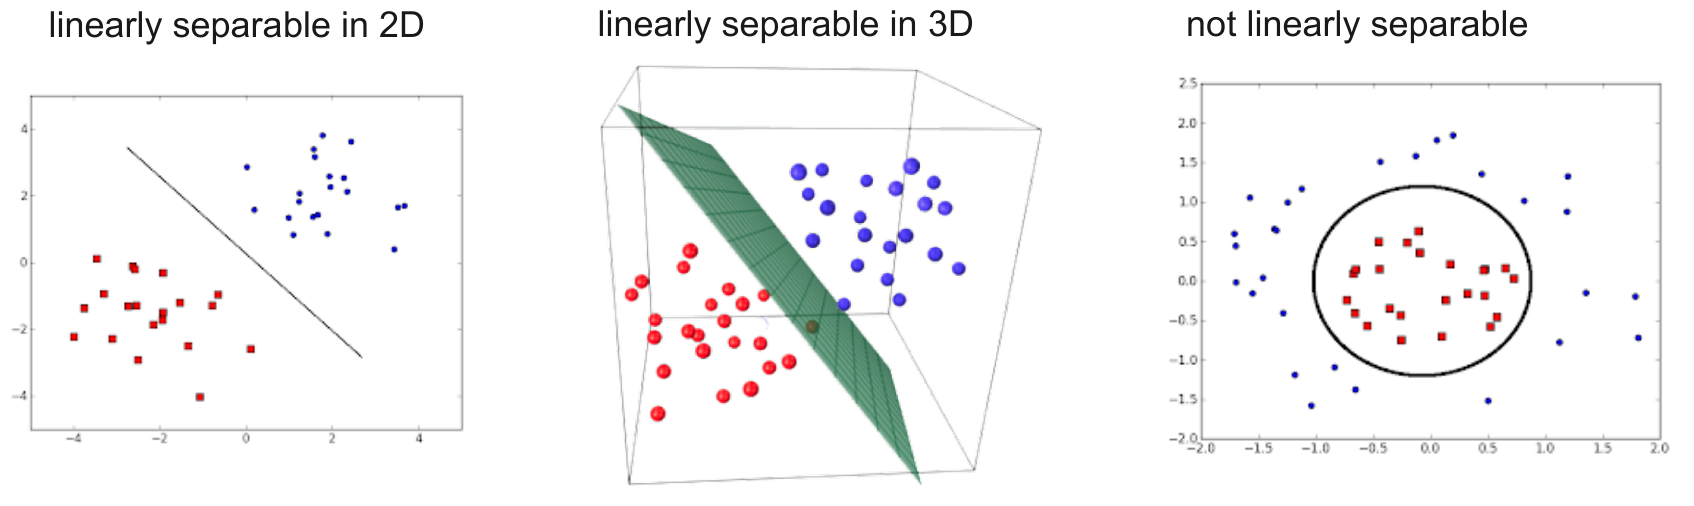
\includegraphics[width=\linewidth]{linear-separability.png}

\subsection{Decision Boundary}
Boundary with two \textbf{features} (bsc grades and workex):\\
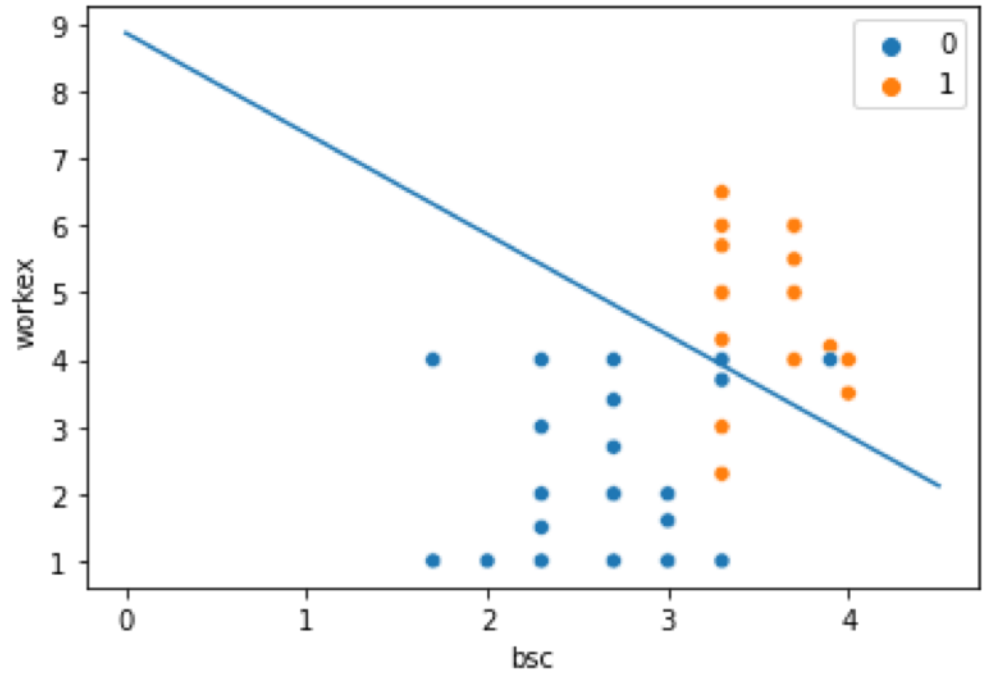
\includegraphics[width=\linewidth]{decision-boundary.png}\\
Use the logistic regression (sigmoid) for calculation of boundary.
If a simple line perfectly separates the classes, then the classes are said to be linearly separable!

\subsection{Multi-class classification}
LR can be extended to multiple classes in some obvious ways.

\subsubsection{One-vs.-rest}
\begin{itemize}
  \item train a single classifier for each class ``c'', with the samples of class ``c'' as positive samples and all other samples as negatives.
  \item Apply all classifiers to an unseen sample x
  \item the classifier reports the highest p is the class
\end{itemize}

\subsubsection{One-vs.-one}
\begin{itemize}
  \item Train classifiers to distinguish between each pair of classes (c1,c2), (c1, c3), (c1,c4), (c2, c3), (c2, c4), (c3,c4).
  \item Apply all classifiers to an unseen sample x.
  \item Combine the results to produce final classification.
\end{itemize}

\subsection{KNN classification}
A datapoint is known by the company it keeps.\\
Given a test data point, KNN:
\begin{itemize}
  \item computes k nearest neighbours of it,
  \item returns the most frequent class of the $k$ neighbours
\end{itemize}
For this, \textbf{all} distances to all points have to be calculated.
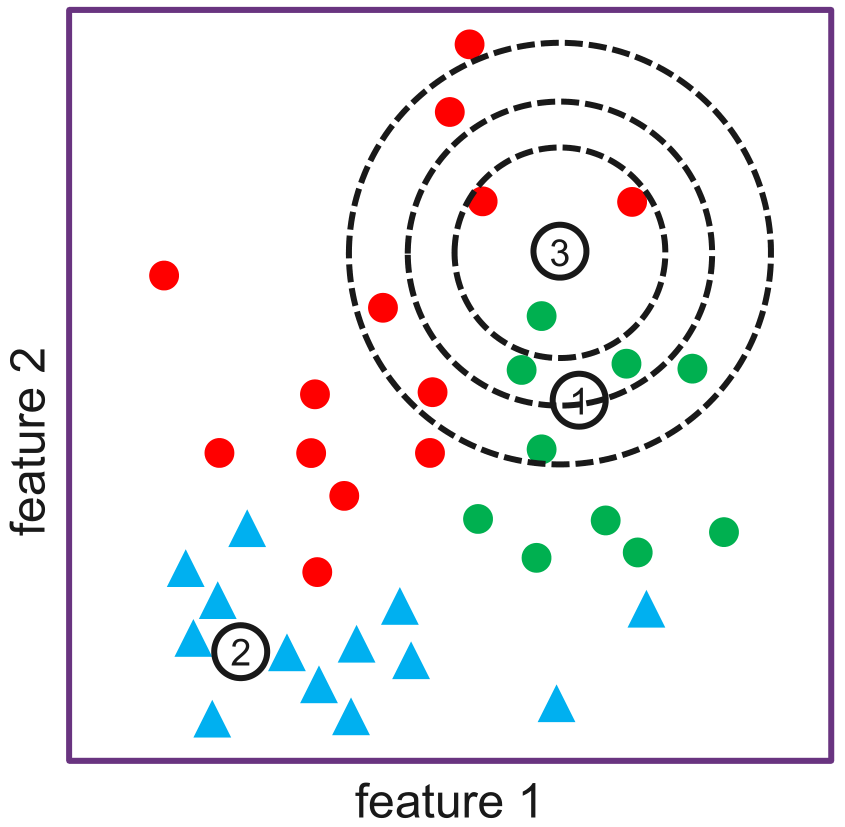
\includegraphics[width=0.7\linewidth]{knn-classification.png}

\subsection{KNN Details}
\begin{enumerate}
  \item Load the training as well as test data.
  \item Choose the value of $k$
  \item For each test data points $x_{test}$
  \begin{enumerate}
    \item For all training data $x_{train}$, calculate the $d(x_{test},x_{train})$
    \item Sort training data in the ascending order of the distance
    \item Choose the first $k$ data points from the sorted training data
    \item Choose the most frequently occurring class from the $k$ data points as the classification result
  \end{enumerate}
\end{enumerate}

\subsubsection{Distance Metric}
\textbf{Cosine Distance}: See Week 2\\
\textbf{Manhattan Distance}: $d_M = \displaystyle\sum_{i = 1}^{n}|X_{1,n} - X_{2,n}|$\\
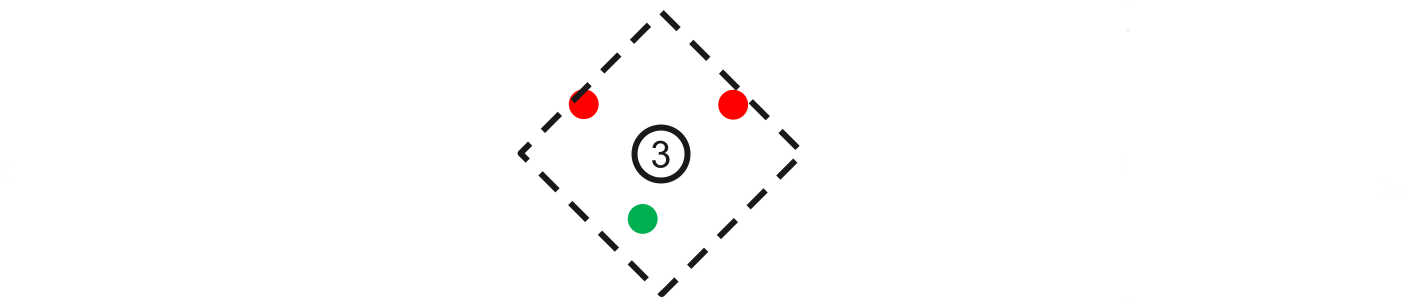
\includegraphics[width=\linewidth]{manhatten-distance.png}\\
\textbf{Euclidean Distance}: $d_E = \sqrt{\displaystyle\sum_{i = 1}^{n}(X_{1,n} - X_{2,n})^2}$\\
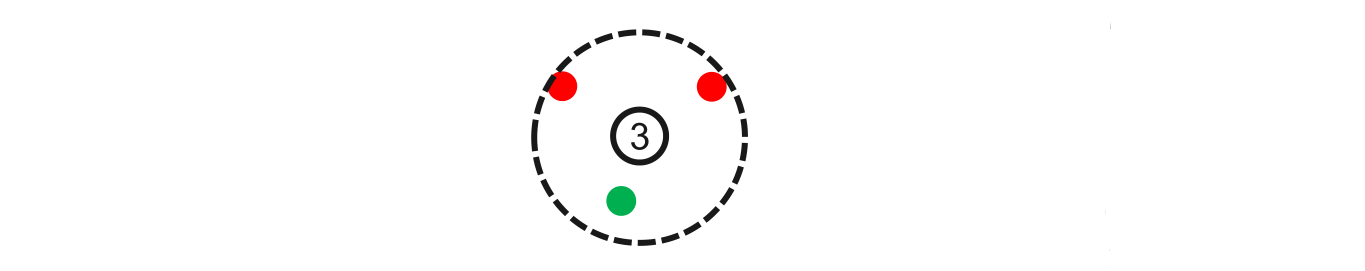
\includegraphics[width=\linewidth]{euclidean-distance.png}\\
